\documentclass[letterpaper]{article}
\usepackage[submission]{aaai2027}
\usepackage[hyphens]{url}
\usepackage{graphicx}
\urlstyle{rm}
\def\UrlFont{\rm}
\usepackage{natbib}
\usepackage{caption}
\frenchspacing
\usepackage{amsmath}
\usepackage{amssymb}
\usepackage{booktabs}
\usepackage{xcolor}
\usepackage{float}
\usepackage{pgfplots}
% Shared publication style for every quantitative and conceptual figure.
% Color semantics are fixed across the paper:
%   blue = balanced / position-robust behavior
%   coral = confounded / shortcut-sensitive behavior
%   sand = transition or intermediate state
%   gray = reference or secondary diagnostic
\definecolor{fig-balanced}{HTML}{4E8D96}
\definecolor{fig-confounded}{HTML}{C96F5F}
\definecolor{fig-transition}{HTML}{D8C58D}
\definecolor{fig-neutral}{HTML}{8C8C96}
\definecolor{fig-ink}{HTML}{303840}
\definecolor{fig-light}{HTML}{F4F7F8}

\usetikzlibrary{arrows.meta,positioning,calc}
\pgfplotsset{
    compat=1.18,
    expplot/.style={
        width=\columnwidth,
        tick label style={font=\footnotesize, text=fig-ink},
        xlabel style={font=\footnotesize, text=fig-ink},
        ylabel style={font=\footnotesize, text=fig-ink},
        legend style={font=\footnotesize, draw=none, cells={anchor=west}},
        every axis plot/.append style={line width=1.0pt, mark size=2.6pt},
        tick style={draw=fig-ink, line width=0.45pt},
        axis line style={draw=fig-ink, line width=0.55pt},
        axis lines=left,
    },
    expgrid/.style={
        ymajorgrids=true,
        grid style={draw=fig-neutral!18, line width=0.4pt},
    },
}


\newcommand{\acc}{\textsc{Acc}}
\newcommand{\con}{\textsc{Con}}
\newcommand{\ccal}{\textsc{Cal}}
\newcommand{\multirow}[3]{#3}
\providecommand{\href}[2]{#2}
\pdfinfo{
/TemplateVersion (2027.1)
}
\setcounter{secnumdepth}{0}

\title{Supplementary Material: When Accuracy Follows Position}

\author{Anonymous Submission}
\affiliations{}

\begin{document}
\tolerance=1500
\emergencystretch=3em
\hbadness=3000
\maketitle

\section*{Supplementary Material}
This document provides additional training details, data construction information, robustness controls, cross-model results, and extended analyses for the main paper.

\appendix
\section{Training Details}
\label{app:training}

Table~\ref{tab:hparams} lists the shared training hyperparameters used unless otherwise stated.

\textbf{Reward definitions.} The accuracy reward is binary label match: $R_{\text{acc}} = \mathbb{1}[v = v^*]$. The decisiveness proxy is $R_{\text{dec}} = 0.5\,\mathbb{1}[v \neq \mathrm{C}]$. The confidence proxy is a Brier-shaped score $R_{\text{conf}} = 1-(\tilde c-\mathbb{1}[v=v^*])^2$, where the parser uses an emitted confidence if present and otherwise sets $\tilde c=0.8$ for A/B or $0.5$ for C. The composite reward is $R = \alpha R_{\text{acc}} + \beta R_{\text{dec}} + \gamma R_{\text{conf}}$, with $\alpha=1.0$, $\beta=0.5$, and $\gamma=0.3$. Because the prompt requests only a verdict and none of the 119 saved evaluation summaries records an explicit confidence, we treat this component as a fixed-confidence proxy, not a calibration measure.

\begin{table}[H]
\centering
\footnotesize
\begin{tabular}{ll}
\toprule
\textbf{Hyperparameter} & \textbf{Value} \\
\midrule
Base model & Qwen2.5-7B-Instruct \\
LoRA rank / $\alpha$ & 64 / 128 \\
Target modules & q, k, v, o projections \\
GRPO group size & 8 \\
Batch size & 4 (grad accum 4) \\
Learning rate & $5 \times 10^{-6}$ (default) \\
LR scheduler & Cosine decay \\
Max prompt / response & 2048 / 1024 tokens \\
Training steps & 500 (primary Qwen2.5) \\
Reward weights & 1.0, 0.5, 0.3 \\
Seeds & 42, 123, 456, 789 \\
Hardware & 1$\times$ H200 (143GB) per run \\
Training time & $\sim$2.5h per run \\
\bottomrule
\end{tabular}
\caption{Primary Qwen2.5 training hyperparameters. For the learning-rate study, we additionally test $1 \times 10^{-5}$, $3 \times 10^{-6}$, $2 \times 10^{-6}$, and $1 \times 10^{-6}$. Cross-model controls use the run lengths recorded with their released experiment configurations.}
\label{tab:hparams}
\end{table}

\section{Data Construction}
\label{app:data}

RewardBench~\citep{lambert2024rewardbench} provides 2,985 preference pairs drawn from multiple evaluation subsets. With seed 42, we randomly shuffle instance indices and partition them into 2,089 training, 447 reserved validation, and 449 test instances. The validation slice was not saved or used for early stopping, hyperparameter selection, or model selection in the reported runs. For analysis only, we aggregate test subsets into five slices---Chat, Reasoning, Safety, Code, and Adversarial---as detailed in Appendix~\ref{app:domain}. In our unbalanced judge-prompt conversion, the \texttt{chosen} field is rendered as Response A for every training and test instance.

For unbalanced training, we use this data as-is. For balanced training, we include both orientations of each training pair: the original instance with gold label A and a swapped mirror with gold label B. This yields 4,178 balanced training prompts and ensures that position A is preferred in exactly half the training instances. We also run a non-duplicated balanced control with 2,089 prompts in Appendix~\ref{app:dose}.

\textbf{Position bias in preference-data conversion.} The ``always A'' artifact is a property of the conversion rule, not an unavoidable property of RewardBench or the \texttt{chosen}/\texttt{rejected} schema. Any converter that places \texttt{chosen} in a fixed judge-prompt slot creates the confound; randomizing or balancing the slots prevents it. We therefore make no claim that existing pipelines using other preference datasets necessarily contain the same artifact.

For SFT, we pair each judge prompt with a fixed generic rationale template naming the gold slot, followed by ``[[A]]'' or ``[[B]].'' For DPO, the chosen and rejected outputs use the same generic slot-specific templates with the correct and opposite verdicts, respectively. These targets test whether the optimization objective learns the label-position regularity; they are not intended as high-quality rationale supervision.

\textbf{SFT 100\% accuracy sanity check.} The SFT result (100\% original-order accuracy, 0\% consistency on unbalanced data) is extreme but expected. Every target contains both a generic rationale favoring Assistant A and the verdict ``[[A]],'' so either part of the target exposes the same slot regularity. Balanced SFT removes the global constant-label solution by using A and B equally often. Its improvement therefore shows that SFT can learn a rule beyond always selecting one slot; it should not be read as evidence about rationale quality.

For evaluation, we always test both the original and position-swapped version of each test instance, using the swap rate as our consistency metric.

\textbf{Artifact scope.} The anonymous artifact includes the exact conversion, SFT, DPO, GRPO, evaluation, and aggregation scripts; the saved per-example predictions used for every reported table; and a CPU-only command that regenerates the summaries and bootstrap checks. Model checkpoints and licensed source examples are omitted for size and redistribution reasons. Machine-specific paths in stored aggregate metadata are redacted without changing metric values.

\section{Prompt Template}
\label{app:prompt}

The following is the training and evaluation template; line breaks are wrapped for display.
{\scriptsize
\begin{verbatim}
Please act as an impartial judge and evaluate the
quality of the responses provided by two AI
assistants to the user question displayed below.
You should choose the assistant that follows the
user's instructions and answers the user's question
better. Your evaluation should consider factors
such as the helpfulness, relevance, accuracy,
depth, creativity, and level of detail of their
responses.

Begin your evaluation by comparing the two
responses and provide a short explanation. Avoid
any position biases and ensure that the order in
which the responses were presented does not
influence your decision. Do not allow the length
of the responses to influence your evaluation.
Be as objective as possible.

After providing your explanation, output your
final verdict by strictly following this format:
"[[A]]" if assistant A is better, "[[B]]" if
assistant B is better, and "[[C]]" if it is a tie
or you cannot determine a winner.

[User Question]
{question}

[The Start of Assistant A's Answer]
{answer_a}
[The End of Assistant A's Answer]

[The Start of Assistant B's Answer]
{answer_b}
[The End of Assistant B's Answer]
\end{verbatim}
}

\textbf{Output parsing and format handling.} Evaluation parses \texttt{[[A]]}, \texttt{[[B]]}, or \texttt{[[C]]}; a parse failure is counted as incorrect and inconsistent. The parser also accepts an optional numeric confidence, but all 119 saved evaluation summaries report zero explicit-confidence outputs. During GRPO training, an unparseable completion is mapped to C with fallback confidence 0.5; since all training labels are A/B, it receives zero accuracy and decisiveness reward but a confidence-proxy value of 0.75. Ties are treated as self-consistent when both orientations produce C. A stricter tie-as-inconsistent check changes the key trained-model consistency comparisons by at most about one point and does not alter the conclusions.

\section{Prompt and Label Controls}
\label{app:label_controls}

Prompt-level mitigation (``evaluate based on content quality only; ordering is random'') only marginally changes consistency: Qwen2.5 moves from 61.7\% to 63.9\%, while Mistral moves from 20.0\% to 18.9\%. We also evaluate unbalanced-GRPO models with alternative label schemes: ``Response 1/2'' and ``Response Left/Right.'' The shortcut persists across all prompt and label variants and all three model families we test (Table~\ref{tab:labels-app}). Zero parse failures confirm that the Qwen2.5 and Mistral models follow the relabeled format rather than reverting to ``[[A]].'' For Qwen3, the reported prompt/label-control runs use thinking disabled and retain parse failures below 1.3\%; without this setting, parse failures rise to 39--42\% and the control is not interpretable.

\begin{table}[H]
\centering
\scriptsize
\setlength{\tabcolsep}{3pt}
\begin{tabular}{@{}llrrrr@{}}
\toprule
\textbf{Model} & \textbf{Control} & \textbf{Acc} & \textbf{Con} & \textbf{Orig.} & \textbf{Parse} \\
\midrule
\multirow{4}{*}{Qwen2.5} & A/B & 94.0 & 61.7 & 94.0 & 0.0 \\
& Anti & 93.8 & 63.9 & 93.8 & 0.0 \\
& 1 / 2 & 94.7 & 60.8 & 94.7 & 0.0 \\
& L/R & 94.2 & 59.9 & 94.2 & 0.0 \\
\midrule
\multirow{4}{*}{Qwen3} & A/B & 88.4 & 78.8 & 88.4 & 1.1 \\
& Anti & 88.0 & 80.2 & 88.0 & 0.7 \\
& 1 / 2 & 88.4 & 81.7 & 88.4 & 1.2 \\
& L/R & 85.7 & 83.7 & 85.7 & 1.0 \\
\midrule
\multirow{4}{*}{Mistral} & A/B & 98.9 & 20.0 & 98.9 & 0.0 \\
& Anti & 98.7 & 18.9 & 98.7 & 0.0 \\
& 1 / 2 & 99.6 & 12.0 & 99.6 & 0.0 \\
& L/R & 99.1 & 15.6 & 99.1 & 0.0 \\
\bottomrule
\end{tabular}
\caption{Prompt and label controls. Anti is the ordering-randomized anti-shortcut prompt; L/R denotes Left/Right labels. Orig. is original-order first-selection; Parse is the two-order parse-failure rate.}
\label{tab:labels-app}
\end{table}

\section{Evaluation-Time Swap Filtering}
\label{app:posthoc}

Post-hoc swap filtering can identify examples on which the original and swapped predictions disagree, but it does not repair the underlying model on those examples. We keep only pairs whose predictions are logically consistent after swapping positions. This produces a high-accuracy retained subset, but coverage collapses exactly when the shortcut is severe: unbalanced SFT retains 0.0\% of examples, and unbalanced full GRPO retains only 58.7\% (Table~\ref{tab:posthoc}). A random fallback on discarded examples reduces unbalanced full GRPO to 74.9\% expected accuracy, while balanced full GRPO keeps 84.0\% coverage and 82.6\% expected fallback accuracy. Thus swap filtering is useful as a diagnostic or selective abstention rule, but data balancing addresses the source of the shortcut.

\begin{table}[H]
\centering
\scriptsize
\setlength{\tabcolsep}{3pt}
\begin{tabular}{@{}lrrrr@{}}
\toprule
\textbf{Setting} & \textbf{Acc} & \textbf{Cov.} & \textbf{Ret.} & \textbf{Rand.} \\
\midrule
Baseline & 80.2 & 81.5 & 84.2 & 77.8 \\
SFT unbal & 100.0 & 0.0 & -- & 50.0 \\
SFT bal & 91.3 & 87.1 & 96.2 & 90.2 \\
GRPO-A unbal & 94.7 & 59.8 & 92.4 & 75.3 \\
GRPO-F unbal & 94.7 & 58.7 & 92.3 & 74.9 \\
GRPO-F bal & 83.7 & 84.0 & 88.8 & 82.6 \\
\bottomrule
\end{tabular}
\caption{Post-hoc swap filtering on Qwen2.5. Cov. is retained coverage; Ret. is accuracy on retained examples; Rand. assumes a random binary fallback on discarded examples. GRPO rows report seed means.}
\label{tab:posthoc}
\end{table}

\section{Length-Confound Control}
\label{app:length}

To separate position shortcuts from generic shortcut learning, we include a non-positional confound control in which the training preference is correlated with response length rather than response order. This control does not produce the same failure mode: length-confounded GRPO remains close to the untrained baseline in both consistency and first-position rate (Table~\ref{tab:length}). In contrast, position-confounded GRPO-A increases original-order accuracy to 94.7\% while reducing consistency to 59.8\% and pushing the first-position rate to 68.1\%. This suggests that the severe collapse we study is tied to the globally predictive position feature introduced by preference-data conversion, not simply to the presence of any spurious training feature.

\begin{table}[H]
\centering
\scriptsize
\setlength{\tabcolsep}{3pt}
\begin{tabular}{@{}lrrrr@{}}
\toprule
\textbf{Setting} & \textbf{Acc} & \textbf{Swap} & \textbf{Con} & \textbf{First} \\
\midrule
Baseline & 80.2 & 75.3 & 81.5 & 49.3 \\
Position-conf. GRPO-A & 94.7 & 55.7 & 59.8 & 68.1 \\
Length-conf. GRPO & 80.9 & 75.8 & 79.7 & 50.6 \\
\bottomrule
\end{tabular}
\caption{Length-confound control on Qwen2.5. Swap is swapped-order accuracy; First is the two-order first-position rate. The two GRPO rows report \mbox{three-seed means}.}
\label{tab:length}
\end{table}

\section{Cross-Model Validation}
\label{app:crossmodel}

To verify that our findings generalize beyond a single model family, we replicate experiments on Qwen3-8B~\citep{qwen2025qwen3} (a newer-generation Qwen model) and Mistral-7B-Instruct-v0.3~\citep{jiang2023mistral} (a completely different architecture and pre-training corpus from Mistral AI). Table~\ref{tab:crossmodel} reports the full cross-model comparison. For Qwen3, we use the disable-thinking baseline run so that parsing behavior matches the rest of the Qwen3 evaluations.

\begin{table}[H]
\centering
\footnotesize
\begin{tabular}{llcc}
\toprule
\textbf{Method} & \textbf{Data} & \textbf{Acc} & \textbf{Con} \\
\midrule
\multicolumn{4}{l}{\textit{Qwen2.5-7B-Instruct (primary)}} \\
Baseline & --- & 80.2 & 81.5 \\
SFT & unbal & 100.0 & 0.0 \\
DPO & unbal & 94.2 & 54.3 \\
GRPO & unbal & 94.7{\scriptsize$\pm$0.9} & 58.7{\scriptsize$\pm$9.1} \\
SFT & bal & 91.3 & 87.1 \\
GRPO & bal & 83.7{\scriptsize$\pm$1.1} & 84.0{\scriptsize$\pm$0.8} \\
\midrule
\multicolumn{4}{l}{\textit{Qwen3-8B (cross-generation)}} \\
Baseline & --- & 86.0 & 80.4 \\
SFT & unbal & 100.0{\scriptsize$\pm$0.0} & 0.0{\scriptsize$\pm$0.0} \\
DPO & unbal & 89.3 & 81.3 \\
GRPO & unbal & 88.7{\scriptsize$\pm$0.3} & 80.0{\scriptsize$\pm$1.0} \\
SFT & bal & 88.5{\scriptsize$\pm$1.1} & 89.1{\scriptsize$\pm$0.3} \\
DPO & bal & 88.6 & 85.3 \\
GRPO & bal & 87.4{\scriptsize$\pm$0.8} & 82.2{\scriptsize$\pm$0.6} \\
\midrule
\multicolumn{4}{l}{\textit{Mistral-7B-Instruct-v0.3 (cross-family)}} \\
Baseline & --- & 65.7 & 64.8 \\
SFT & unbal & 100.0 & 0.0 \\
SFT & bal & 92.2 & 84.9 \\
GRPO & unbal & 98.4{\scriptsize$\pm$0.4} & 23.0{\scriptsize$\pm$3.6} \\
GRPO & bal & 81.1{\scriptsize$\pm$0.9} & 68.3{\scriptsize$\pm$3.6} \\
\bottomrule
\end{tabular}
\caption{Cross-model validation across three model families. The position shortcut replicates, but severity is model-dependent: Mistral shows the most extreme collapse, Qwen2.5 is intermediate, and Qwen3 shows the mildest GRPO consistency loss under \mbox{disable-thinking evaluation}.}
\label{tab:crossmodel}
\end{table}

Shortcut severity is model-dependent. Mistral-7B has the lowest baseline original-order accuracy (65.7\%) and the largest trained shortcut (98.4\% accuracy, 23.0\% consistency). Qwen2.5-7B (80.2\% baseline) is intermediate (94.7\%/58.7\%), whereas Qwen3-8B has the highest original-order baseline (86.0\%) and much milder GRPO consistency damage (80.4\% baseline $\to$ 80.0\% unbalanced); balanced GRPO reaches 82.2\%. These three observations are consistent with several explanations, including different initial comparison behavior and model-specific optimization response, but they do not identify capability as the cause. The Qwen3 SFT collapse to 0.0\% consistency also shows that mild GRPO sensitivity is not immunity. Balanced data is the more direct intervention because it removes the position-label correlation instead of relying on a particular model--optimizer interaction.

The models also differ in the \emph{speed} of shortcut emergence. Checkpoint-level evaluation shows that Mistral-7B is already strongly position-dependent by step 100 (98.7\% accuracy, 20.3\% consistency), while Qwen2.5-7B changes more gradually through 500 steps (84.6\%/81.7\% at step 100 $\to$ 94.0\%/61.7\% at step 500). Because training schedules and models differ, this comparison is descriptive rather than a controlled estimate of capability effects. Practically, it motivates auditing early checkpoints rather than waiting until the end of training.

A flatter learning-rate sensitivity pattern also appears on Qwen3-8B. Consistency stays in the high-70s to low-80s across its accuracy-reward sweep (Table~\ref{tab:crosslr}), compared with the sharp Qwen2.5-7B decline under the full reward. Because both the model and reward differ, the curves establish configuration-specific sensitivity rather than a pure model-capability effect.

\begin{table}[H]
\centering
\footnotesize
\begin{tabular}{lcccc}
\toprule
\textbf{LR} & \multicolumn{2}{c}{\textbf{Qwen2.5-7B}} & \multicolumn{2}{c}{\textbf{Qwen3-8B}} \\
\cmidrule(lr){2-3} \cmidrule(lr){4-5}
 & Acc & Con & Acc & Con \\
\midrule
1e-6 & 83.7 & 83.3 & 89.1 & 82.4 \\
2e-6 & 85.7 & 81.1 & 87.8 & 81.5 \\
3e-6 & 90.0 & 75.7 & 87.8 & 82.6 \\
5e-6 & 94.0 & 61.7 & 88.4 & 78.8 \\
1e-5 & 98.9 & 38.1 & 90.2 & 78.4 \\
\bottomrule
\end{tabular}
\caption{Cross-model LR sensitivity. The Qwen2.5 sweep uses the full reward, while the Qwen3 sweep uses the accuracy reward; rows are single-seed controls. Qwen2.5 loses about 45 pp of consistency across the range, compared with about 4 pp for Qwen3, but this is not a controlled model-only comparison.}
\label{tab:crosslr}
\end{table}

Multi-objective rewards also fail to reliably restore consistency on Qwen3-8B: the decisiveness proxy raises consistency from 78.8\% to 82.0\%, while the confidence proxy lowers it to 78.0\%. The composite reward remains below balanced GRPO under the tested weights. These results show that the tested proxy rewards are insufficient for this data-level confound across tested configurations.

All experiments use NVIDIA H200 GPUs (143GB). Total compute: approximately 200 H200-GPU-hours across all experiments.

\section{External Check on Published RL-Trained Judges}
\label{app:judgelrm}

As an external check, we evaluate JudgeLRM's publicly released checkpoints~\citep{chen2025judgelrm} with the same position-swap diagnostic (Table~\ref{tab:judgelrm-app}). JudgeLRM-7B achieves 81.3\% original-order accuracy but 66.1\% swap accuracy and 75.7\% consistency, while JudgeLRM-3B achieves 76.8\% original-order accuracy, 55.9\% swap accuracy, and 67.9\% consistency. These results do not imply that all gains in prior judge training are shortcuts; they show that standard accuracy can hide a position-dependent component.

\begin{table}[H]
\centering
\scriptsize
\setlength{\tabcolsep}{2.5pt}
\resizebox{\columnwidth}{!}{%
\begin{tabular}{lccccc}
\toprule
\textbf{Model} & \textbf{Orig Acc} & \textbf{Swap Acc} & \textbf{Con} & \textbf{First-pos} & \textbf{Bias} \\
\midrule
JudgeLRM-7B & 81.3 & 66.1 & 75.7 & 53.1 & 13.4 \\
JudgeLRM-3B & 76.8 & 55.9 & 67.9 & 56.7 & 15.4 \\
\bottomrule
\end{tabular}
}
\caption{Published RL-trained judges also show a position-dependent component under the swap diagnostic. Bias is the always-first minus always-second inconsistent rate.}
\label{tab:judgelrm-app}
\end{table}

\section{Multi-Seed Stability}
\label{app:seeds}

The primary GRPO pattern is stable across random seeds rather than driven by a single run. Table~\ref{tab:seeds} reports individual seed results for representative unbalanced and balanced conditions. Unbalanced runs maintain high original-order accuracy but low consistency and an elevated first-position rate; balanced runs keep consistency high and the first-position rate near neutral.

\begin{table}[H]
\centering
\scriptsize
\begin{tabular}{llccc}
\toprule
\textbf{Method} & \textbf{Seed} & \textbf{Acc} & \textbf{Con} & \textbf{First-pos} \\
\midrule
\multirow{3}{*}{Acc-only unbal} & s1 & 94.4 & 60.8 & 67.4 \\
 & s2 & 95.6 & 51.7 & 72.0 \\
 & s3 & 94.2 & 66.8 & 64.9 \\
\midrule
\multirow{4}{*}{Full unbal} & s1 & 94.0 & 61.7 & 67.4 \\
 & s2 & 96.0 & 45.2 & 75.3 \\
 & s3 & 94.2 & 63.7 & 66.5 \\
 & s4 & 94.4 & 64.4 & 66.1 \\
\midrule
\multirow{5}{*}{Full bal} & s1 & 84.6 & 85.3 & 50.1 \\
 & s2 & 82.2 & 83.7 & 48.6 \\
 & s3 & 84.4 & 83.3 & 51.3 \\
 & s4 & 82.9 & 83.7 & 49.4 \\
 & s5 & 84.4 & 84.0 & 50.3 \\
\bottomrule
\end{tabular}
\caption{Per-seed results for Qwen2.5 GRPO. Balanced training consistently keeps position-swap consistency high and the first-position rate near 50\%.}
\label{tab:seeds}
\end{table}

\section{Statistical Uncertainty Checks}
\label{app:uncertainty}

We add local uncertainty checks for the main diagnostic effects (Table~\ref{tab:uncertainty}). For single-run SFT comparisons, we use paired bootstrap resampling over the 449 matched test examples. For multi-seed GRPO comparisons, we bootstrap the available seed means; these intervals are descriptive because the number of seeds is small.

\begin{table}[H]
\centering
\scriptsize
\setlength{\tabcolsep}{3pt}
\resizebox{\columnwidth}{!}{%
\begin{tabular}{llcc}
\toprule
\textbf{Comparison} & \textbf{Metric} & \textbf{Diff} & \textbf{95\% CI} \\
\midrule
SFT unbal $\to$ SFT bal & Con & +87.1 & [84.0, 90.0] \\
SFT unbal $\to$ SFT bal & First-pos & -48.9 & [-50.6, -47.2] \\
Baseline $\to$ SFT bal & Avg & +12.5 & [9.5, 15.6] \\
Baseline $\to$ SFT bal & Con & +5.6 & [1.1, 10.0] \\
Qwen2.5 GRPO unbal $\to$ bal & Con & +25.3 & [19.8, 34.4] \\
Qwen2.5 GRPO unbal $\to$ bal & Avg & +7.8 & [5.3, 11.6] \\
Qwen3 GRPO unbal $\to$ bal & Con & +2.2 & [1.1, 3.3] \\
Mistral GRPO unbal $\to$ bal & Con & +45.2 & [40.4, 50.1] \\
\bottomrule
\end{tabular}
}
\caption{Bootstrap uncertainty checks. Diff is after $-$ before in percentage points. Single-run SFT rows use paired-instance bootstrap; multi-seed GRPO rows use seed-mean bootstrap.}
\label{tab:uncertainty}
\end{table}

The intervals support the paper's qualitative interpretation without requiring stronger statistical language. The SFT shortcut collapse and recovery are much larger than instance-level uncertainty, including a 12.5-point gain in order-averaged accuracy over the baseline. For Qwen2.5 GRPO, balancing improves both consistency and order-averaged accuracy; the latter gain is 7.8 points with a descriptive seed-mean interval of [5.3, 11.6]. For Mistral GRPO, the consistency gain is large, whereas the Qwen3 gain is small but positive under the local bootstrap, matching the conclusion that shortcut severity is model- and configuration-dependent.

\section{Learning Rate Sensitivity}
\label{app:lr}

The complete learning rate data is shown in Table~\ref{tab:lr} and visualized in Figure~\ref{fig:lr}.

\begin{figure}[H]
\centering
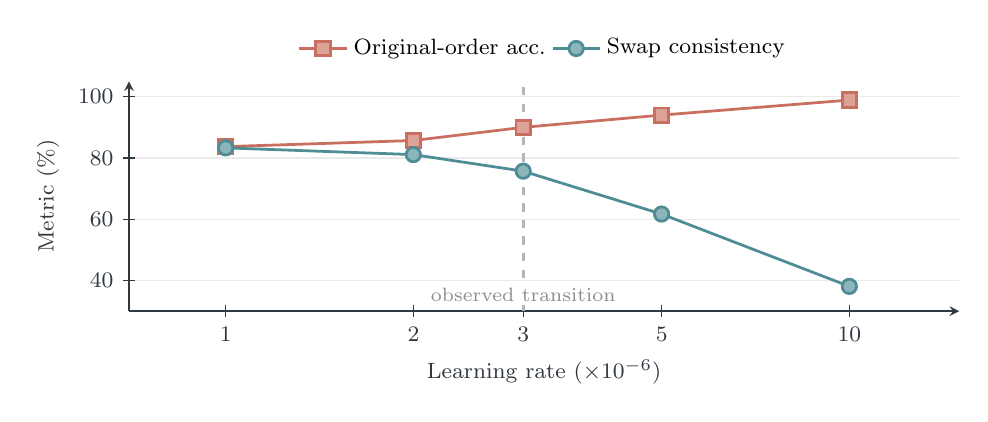
\begin{tikzpicture}
\begin{axis}[
    expplot,
    expgrid,
    height=4.5cm,
    xlabel={Learning rate ($\times 10^{-6}$)},
    ylabel={Metric (\%)},
    xmode=log,
    xmin=7e-7, xmax=1.5e-5,
    ymin=30, ymax=105,
    xtick={1e-6, 2e-6, 3e-6, 5e-6, 1e-5},
    xticklabels={1, 2, 3, 5, 10},
    ytick={40,60,80,100},
    legend style={at={(0.5,1.05)}, anchor=south, legend columns=2},
    clip=false,
]
\addplot[fig-confounded, mark=square*, mark options={fill=fig-confounded!65, draw=fig-confounded}] coordinates {(1e-6,83.7) (2e-6,85.7) (3e-6,90.0) (5e-6,94.0) (1e-5,98.9)};
\addlegendentry{Original-order acc.}
\addplot[fig-balanced, mark=*, mark options={fill=fig-balanced!65, draw=fig-balanced}] coordinates {(1e-6,83.3) (2e-6,81.1) (3e-6,75.7) (5e-6,61.7) (1e-5,38.1)};
\addlegendentry{Swap consistency}
\addplot[fig-neutral!65, dashed, forget plot] coordinates {(3e-6,30) (3e-6,105)};
\node[font=\scriptsize, anchor=south, text=fig-neutral, fill=white, inner sep=1pt] at (axis cs:3e-6,32) {observed transition};
\end{axis}
\end{tikzpicture}
\caption{Learning-rate sensitivity in the single-seed Qwen2.5 full-reward sweep. Original-order accuracy rises as position-swap consistency falls; no uncertainty is shown because each point is one run. The dashed marker denotes an observed transition region in this grid, not an estimated universal threshold.}
\label{fig:lr}
\end{figure}

\begin{table}[H]
\centering
\footnotesize
\begin{tabular}{lccc}
\toprule
\textbf{Learning Rate} & \textbf{Acc} & \textbf{Con} & \textbf{First-pos} \\
\midrule
Baseline & 80.2 & 81.5 & 49.3 \\
1e-6 & 83.7 & 83.3 & 51.0 \\
2e-6 & 85.7 & 81.1 & 54.3 \\
3e-6 & 90.0 & 75.7 & 58.2 \\
5e-6 (standard) & 94.0 & 61.7 & 67.4 \\
1e-5 & 98.9 & 38.1 & 80.5 \\
\bottomrule
\end{tabular}
\caption{Full learning rate sweep. First-position rate increases with training intensity as consistency falls.}
\label{tab:lr}
\end{table}
\section{Training Algorithm Controls}
\label{app:sft}

The position shortcut is not specific to any training paradigm. SFT on unbalanced data achieves 100\% accuracy with 0\% consistency. DPO falls between SFT and GRPO in severity (94.2\%/54.3\%). GRPO retains partial consistency (58.7\% multi-seed mean). The observed ordering SFT $>$ DPO $>$ GRPO describes shortcut severity in this configuration, but it does not isolate an optimizer-level mechanism; all three objectives remain vulnerable to the position-label confound.

When given balanced data, SFT achieves higher original-order accuracy (91.3\% versus 84.6\% for GRPO in the corresponding single run), showing that direct supervision can use deconfounded labels effectively in this setting. The same SFT procedure collapses under unbalanced labels, so this comparison supports sensitivity to data construction rather than a claim about relative data efficiency or optimizer mechanism.

\section{Cross-Model Learning Rate Sensitivity}
\label{app:crosslr}

Figure~\ref{fig:crosslr} shows a much flatter learning-rate curve for the tested Qwen3-8B accuracy-reward configuration. Since the Qwen2.5 curve uses the full reward, the comparison does not isolate model family from reward setup.

\begin{figure}[H]
\centering
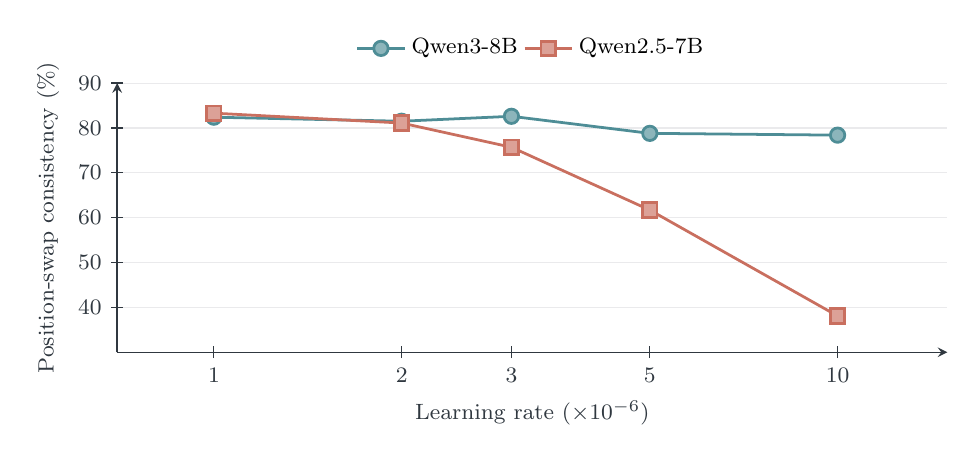
\begin{tikzpicture}
\begin{axis}[
    expplot,
    expgrid,
    height=5cm,
    xlabel={Learning rate ($\times 10^{-6}$)},
    ylabel={Position-swap consistency (\%)},
    xmode=log,
    xmin=7e-7, xmax=1.5e-5,
    ymin=30, ymax=90,
    xtick={1e-6, 2e-6, 3e-6, 5e-6, 1e-5},
    xticklabels={1, 2, 3, 5, 10},
    ytick={40,50,60,70,80,90},
    legend style={at={(0.5,1.05)}, anchor=south, legend columns=2},
]
\addplot[fig-balanced, mark=*, mark options={fill=fig-balanced!65, draw=fig-balanced}] coordinates {(1e-6,82.4) (2e-6,81.5) (3e-6,82.6) (5e-6,78.8) (1e-5,78.4)};
\addlegendentry{Qwen3-8B}
\addplot[fig-confounded, mark=square*, mark options={fill=fig-confounded!65, draw=fig-confounded}] coordinates {(1e-6,83.3) (2e-6,81.1) (3e-6,75.7) (5e-6,61.7) (1e-5,38.1)};
\addlegendentry{Qwen2.5-7B}
\end{axis}
\end{tikzpicture}
\caption{Position-swap consistency across two single-seed learning-rate sweeps. Qwen2.5-7B loses about 45 pp under the full reward, whereas Qwen3-8B changes by about 4 pp under the accuracy reward. Each point is one run, and the differing rewards preclude a model-only causal comparison.}
\label{fig:crosslr}
\end{figure}

The contrast shows that shortcut sensitivity is not constant across tested configurations. Qwen3-8B maintains higher consistency under moderate learning rates in its accuracy-reward sweep, but its curve should not be interpreted as evidence that scaling caused the difference. The practical conclusion is narrower: every model and training recipe still requires a position-swap audit.

\section{Multi-Objective Reward Analysis}
\label{app:reward}

A key question is whether reward engineering can substitute for data deconfounding. We test three reward configurations on both models (all on unbalanced data). For Qwen2.5-7B, rows report seed means where available; Qwen3-8B rows are single-seed reward controls.

\begin{table}[H]
\centering
\footnotesize
\begin{tabular}{lcccc}
\toprule
\textbf{Reward} & \multicolumn{2}{c}{\textbf{Qwen2.5-7B}} & \multicolumn{2}{c}{\textbf{Qwen3-8B}} \\
\cmidrule(lr){2-3} \cmidrule(lr){4-5}
 & Acc & Con & Acc & Con \\
\midrule
Accuracy only & 94.7 & 59.8 & 88.4 & 78.8 \\
+ Decisive & 93.9 & 66.3 & 88.2 & 82.0 \\
+ Confidence proxy & 95.4 & 56.1 & 89.1 & 78.0 \\
Full composite & 94.7 & 58.7 & 87.8 & 80.8 \\
\bottomrule
\end{tabular}
\caption{Reward ablation across models. Qwen2.5 rows use multi-seed means where available, while Qwen3 rows are single-seed controls. No proxy reward exceeds balanced data (Qwen2.5 GRPO balanced: 84.0\% con, Qwen3 GRPO balanced: 82.2\% con). The fixed-confidence proxy lowers consistency on \mbox{both models}.}
\label{tab:reward_ablation}
\end{table}

The tested proxy rewards do not replace data deconfounding (Table~\ref{tab:reward_ablation}). The decisiveness proxy penalizes tie hedging but cannot distinguish content-based decisiveness from following the position shortcut. The fixed-confidence proxy lowers consistency on both models because, with verdict-only outputs, it is almost a deterministic transformation of the predicted label and correctness rather than an independent calibration signal. Overall, these components help only partially and do not match the direct intervention of removing the position-label correlation from the training data.

\section{Training Dynamics Details}
\label{app:dynamics}

Table~\ref{tab:dynamics} gives the paired checkpoint-level data for the training dynamics experiment. At these shared checkpoints, original-order accuracy and the first-position rate increase as training proceeds, while consistency is preserved only at the earliest checkpoint and then drops sharply. The composite reward follows the same shortcut trajectory rather than materially slowing the collapse.

\begin{center}
\begin{minipage}{\columnwidth}
\centering
\resizebox{\columnwidth}{!}{%
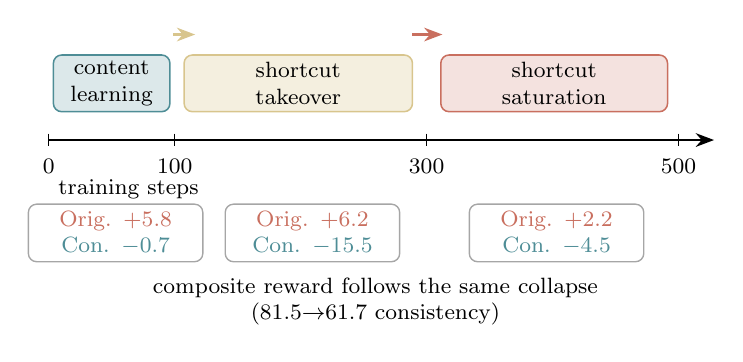
\begin{tikzpicture}[
    font=\footnotesize,
    >=Stealth,
    phase/.style={draw, line width=0.55pt, rounded corners=3pt, align=center, minimum height=0.72cm, inner sep=2pt},
    chip/.style={draw=black!35, fill=white, line width=0.5pt, rounded corners=3pt, align=center, inner sep=2.5pt, text width=2.04cm},
    axis/.style={-Stealth, thick, draw=black}
]
\draw[axis] (0,0) -- (8.45,0);
\foreach \x/\label in {0/0,1.6/100,4.8/300,8.0/500} {
    \draw[black] (\x,0.08) -- (\x,-0.08);
    \node[anchor=north, text=black] at (\x,-0.12) {\label};
}
\node[anchor=west, font=\footnotesize] at (0,-0.62) {training steps};

\draw[draw=fig-balanced, fill=fig-balanced!20, line width=0.55pt, rounded corners=3pt] (0.06,0.36) rectangle (1.54,1.08);
\draw[draw=fig-transition, fill=fig-transition!28, line width=0.55pt, rounded corners=3pt] (1.72,0.36) rectangle (4.62,1.08);
\draw[draw=fig-confounded, fill=fig-confounded!20, line width=0.55pt, rounded corners=3pt] (4.98,0.36) rectangle (7.86,1.08);
\node[align=center] at (0.80,0.72) {content\\learning};
\node[align=center] at (3.17,0.72) {shortcut\\takeover};
\node[align=center] at (6.42,0.72) {shortcut\\saturation};

\node[chip] at (0.85,-1.18) {\textcolor{fig-confounded}{Orig. $+5.8$}\\\textcolor{fig-balanced}{Con. $-0.7$}};
\node[chip] at (3.35,-1.18) {\textcolor{fig-confounded}{Orig. $+6.2$}\\\textcolor{fig-balanced}{Con. $-15.5$}};
\node[chip] at (6.45,-1.18) {\textcolor{fig-confounded}{Orig. $+2.2$}\\\textcolor{fig-balanced}{Con. $-4.5$}};

\draw[->, thick, draw=fig-transition] (1.58,1.34) -- (1.86,1.34);
\draw[->, thick, draw=fig-confounded] (4.62,1.34) -- (5.00,1.34);
\node[align=center, font=\footnotesize, text=black] at (4.15,-2.05) {composite reward follows the same collapse\\(81.5$\to$61.7 consistency)};
\end{tikzpicture}
}
\captionsetup{hypcap=false,justification=raggedright,singlelinecheck=false}
\captionof{figure}{Single-seed checkpoint dynamics for accuracy-only GRPO. Early training raises original-order accuracy with little consistency loss; the middle checkpoints show shortcut takeover, and the final phase approaches a position-dependent policy. Phase boundaries summarize the observed checkpoints rather than estimated change points.}
\label{fig:dynamics}
\end{minipage}
\end{center}

\begin{center}
\begin{minipage}{\columnwidth}
\centering
\footnotesize
\begin{tabular}{lcccccc}
\toprule
\textbf{Steps} & \multicolumn{3}{c}{\textbf{Acc-only}} & \multicolumn{3}{c}{\textbf{Full}} \\
\cmidrule(lr){2-4} \cmidrule(lr){5-7}
 & Acc & Con & First & Acc & Con & First \\
\midrule
0 (base) & 80.2 & 81.5 & 49.3 & 80.2 & 81.5 & 49.3 \\
100 & 86.0 & 80.8 & 53.8 & 84.6 & 81.7 & 53.5 \\
200 & 89.1 & 76.8 & 57.1 & 90.9 & 74.6 & 59.8 \\
300 & 92.2 & 65.3 & 63.7 & 93.5 & 65.9 & 64.9 \\
500 & 94.4 & 60.8 & 67.4 & 94.0 & 61.7 & 67.4 \\
\bottomrule
\end{tabular}
\captionsetup{hypcap=false}
\captionof{table}{Training dynamics at paired checkpoints. Original-order accuracy and the first-position rate increase together, while position-swap consistency drops after the earliest checkpoint. The composite reward reaches nearly the same endpoint as the \mbox{accuracy-only reward}.}
\label{tab:dynamics}
\end{minipage}
\end{center}

\section{Per-Domain Analysis}
\label{app:domain}

Each domain's vulnerability to the shortcut varies substantially (Table~\ref{tab:domain}). We report the primary Qwen2.5 GRPO full setting by domain, using seed means for the unbalanced and balanced rows. The shortcut appears in every domain, but reasoning shows the cleanest collapse: unbalanced GRPO reaches 98.6\% original-order accuracy while consistency falls to 19.6\% and the first-position rate rises to 90.2\%. Balanced training moves this rate back toward neutral and recovers consistency in all domains. Because the smallest slices contain only 43--69 examples, these results are diagnostic rather than independent domain conclusions.

\begin{center}
\begin{minipage}{\columnwidth}
\centering
\footnotesize
\setlength{\tabcolsep}{3pt}
\begin{tabular}{llccccc}
\toprule
\textbf{Setting} & \textbf{Metric} & \textbf{Chat} & \textbf{Reas.} & \textbf{Safe} & \textbf{Code} & \textbf{Adv.} \\
\midrule
\multirow{3}{*}{Baseline} & A & 96.6 & 78.3 & 80.9 & 85.2 & 32.6 \\
 & C & 93.1 & 63.8 & 90.4 & 78.5 & 72.1 \\
 & F & 51.1 & 60.1 & 48.3 & 45.2 & 44.2 \\
\midrule
\multirow{3}{*}{Unbal.} & A & 99.4 & 98.6 & 94.1 & 96.3 & 75.0 \\
 & C & 64.9 & \textbf{19.6} & 73.7 & 64.4 & 51.2 \\
 & F & 67.1 & \textbf{90.2} & 62.5 & 63.0 & 73.3 \\
\midrule
\multirow{3}{*}{Bal.} & A & 94.3 & 85.5 & 82.6 & 91.3 & 38.6 \\
 & C & 91.5 & 70.7 & 88.7 & 84.1 & 77.2 \\
 & F & 50.6 & 58.6 & 48.8 & 47.9 & 44.4 \\
\bottomrule
\end{tabular}
\captionsetup{hypcap=false}
\captionof{table}{Per-domain Qwen2.5 GRPO full diagnostics. A is original-order accuracy, C is position-swap consistency, and F is the two-order first-position rate. Unbalanced and balanced rows report seed means. Domain sizes are Chat 87, Reasoning 69, Safety 115, Code 135, and Adversarial 43.}
\label{tab:domain}
\end{minipage}
\end{center}

\section{Stylized Slot-Bias Derivation}
\label{app:slotbias}

The functional argument in the main text can be made explicit with a deliberately simple discriminative model. Let $y \in \{+1,-1\}$ denote whether the first or second response is preferred, and write the judge logit as
\[
f_\theta(x)=d_\theta(x)+b,
\]
where $d_\theta(x)$ summarizes content-comparison evidence and $b$ is a global first-position bias. Under logistic loss,
\[
\mathcal{L}=\mathbb{E}_{(x,y)}
\left[\log\!\left(1+\exp\!\left(-y(d_\theta(x)+b)\right)\right)\right],
\]
the derivative with respect to the position term is
\[
\frac{\partial \mathcal{L}}{\partial b}
=-\mathbb{E}_{(x,y)}
\left[y\,\sigma\!\left(-y(d_\theta(x)+b)\right)\right].
\]
Near initialization, with $d_\theta(x)\approx0$ and $b\approx0$, $\sigma(0)=1/2$. If $\alpha=\Pr(y=+1)$, then
\[
\frac{\partial \mathcal{L}}{\partial b}
\approx-\frac{1}{2}\mathbb{E}[y]
=-\frac{1}{2}(2\alpha-1).
\]
When every preferred answer is in the first slot ($\alpha=1$), gradient descent therefore increases $b$. When positions are balanced ($\alpha=0.5$), this first-order global shortcut direction vanishes. This calculation is an explanatory local model, not a GRPO derivation or evidence that the trained transformer has one scalar bias.

\section{Confound-Ratio and Data Duplication Control}
\label{app:dose}

We verify that the balanced training fix does not depend on data duplication. Our standard balanced construction creates a mirror of each instance with swapped positions, doubling the dataset from 2,089 to 4,178 training pairs. To control for this size difference, we also train on non-duplicated balanced data (2,089 instances, each randomly assigned to either its original or swapped position with equal probability). The non-duplicated run yields near-identical original-order accuracy and position-swap consistency to the mirrored balanced seed mean (83.1\%/82.6\% versus 83.7\%/84.0\%), with the first-position rate still near neutral (50.2\%). Thus the improvement is attributable to deconfounding rather than data duplication.

We also train at intermediate confound ratios. Figure~\ref{fig:dose} reports consistency loss relative to the balanced reference as the share of position-A preferred examples increases from 50\% to 100\%. The 50\% reference and 100\% endpoint use multi-seed means, whereas the intermediate ratios are single-seed diagnostics. Those intermediate values are non-monotonic, so we interpret the sweep as a boundary diagnostic rather than evidence of a smooth dose-response relation. The clearest result is the sharp deterioration at the fully unbalanced endpoint.

\begin{figure}[H]
\centering
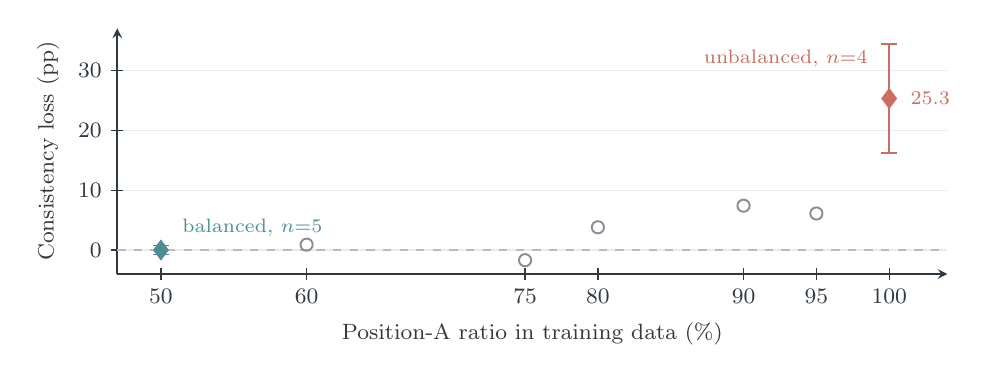
\begin{tikzpicture}
\begin{axis}[
    expplot,
    expgrid,
    height=4.7cm,
    xlabel={Position-A ratio in training data (\%)},
    ylabel={Consistency loss (pp)},
    xmin=47, xmax=104,
    ymin=-4, ymax=37,
    xtick={50,60,75,80,90,95,100},
    xticklabels={50,60,75,80,90,95,100},
    ytick={0,10,20,30},
    clip=false,
]
\addplot[fig-neutral!60, dashed, line width=0.7pt, forget plot] coordinates {(47,0) (104,0)};
\addplot[
    only marks,
    mark=o,
    mark size=2.2pt,
    draw=fig-neutral,
    fill=white,
    line width=0.7pt,
    forget plot
] coordinates {(60,0.9) (75,-1.7) (80,3.8) (90,7.4) (95,6.1)};
\addplot[
    only marks,
    mark=diamond*,
    mark size=3.0pt,
    color=fig-balanced,
    forget plot,
    error bars/.cd,
    y dir=both,
    y explicit,
    error bar style={line width=0.8pt}
] coordinates {(50,0.0) +- (0,0.8)};
\addplot[
    only marks,
    mark=diamond*,
    mark size=3.0pt,
    color=fig-confounded,
    forget plot,
    error bars/.cd,
    y dir=both,
    y explicit,
    error bar style={line width=0.8pt}
] coordinates {(100,25.3) +- (0,9.1)};
\node[font=\scriptsize, text=fig-balanced, anchor=south west] at (axis cs:50.8,0.7) {balanced, $n{=}5$};
\node[font=\scriptsize, text=fig-confounded, anchor=north east] at (axis cs:99.2,35.0) {unbalanced, $n{=}4$};
\node[font=\scriptsize, text=fig-confounded, anchor=west] at (axis cs:100.8,25.3) {25.3};
\end{axis}
\end{tikzpicture}
\caption{Confound-ratio diagnostic measured as consistency loss from the balanced reference. Diamonds are multi-seed endpoint means with seed standard deviation; hollow circles are single-seed intermediate diagnostics and are intentionally not connected. The intermediate values are non-monotonic, while the fully unbalanced endpoint shows the sharp deterioration.}
\label{fig:dose}
\end{figure}

\section{Sharp-Transition Analysis}
\label{app:threshold}

The single-seed Qwen2.5 learning-rate sweep shows a sharp transition within the tested grid rather than uniform degradation (Figure~\ref{fig:lr}). At low rates, consistency remains close to the baseline; at larger rates, original-order accuracy rises while consistency falls. The sparse grid does not identify a critical threshold, but shows that conclusions at one learning rate need not transfer.

The Qwen3-8B accuracy-reward sweep is flatter, maintaining high-70s to low-80s consistency and reaching 78.4\% at the largest rate (Table~\ref{tab:crosslr}). Because the reward setups differ, this is a robustness check rather than a direct attribution to model capability. Practitioners should therefore audit each deployed model--reward--learning-rate combination.

\bibliography{custom}

\end{document}
